	\documentclass[a4paper,11pt,french]{article}
\usepackage[utf8]{inputenc}

\usepackage[T1]{fontenc}
\usepackage[francais]{babel} 
\usepackage[top=1.5cm, bottom=2cm, left=1.5cm, right=1.5cm, includeheadfoot]{geometry} %pour les marges
\usepackage{lmodern}
\usepackage{pict2e}
\usepackage{tikz}	
\usepackage{tikz-uml}
\usepackage{fancyhdr} % Required for custom headers
\usepackage{lastpage} % Required to determine the last page for the footer
\usepackage{extramarks} % Required for headers and footers
\usepackage{graphicx} % Required to insert images
\usepackage{tabularx, longtable}
\usepackage{color, colortbl}
\usepackage{lscape}
\usepackage[hidelinks]{hyperref}
\usepackage{longtable}
\usepackage{multirow}
\usepackage{rotating}
\usepackage{pgfgantt}
\usepackage{pgfcalendar}
\usepackage{ifthen}
\usepackage{gensymb}
\usepackage{color, colortbl}

\usepackage{cmbright}
\usepgflibrary{arrows} % for pgf-umlsd

\linespread{1.1} % Line spacing

% Set up the header and footer
\pagestyle{fancy}
\lhead{\textbf{\hmwkClass -- \hmwkSubject \\ \hmwkTitle \\ \hmwkDocName}} % Top left header
\rhead{
\includegraphics[width=10em]{logo_univ.png}}
\lfoot{\lastxmark} % Bottom left footer
\cfoot{} % Bottom center footer
\rfoot{Page\ \thepage\ / \pageref{LastPage}} % Bottom right footer
\renewcommand\headrulewidth{0.4pt} % Size of the header rule
\renewcommand\footrulewidth{0.4pt} % Size of the footer rule

\setlength{\headheight}{40pt}

\newcommand{\hmwkTitle}{Audit des implantations SSL/TLS} % Assignment title
\newcommand{\hmwkClass}{Master 2 SSI } % Course/class
\newcommand{\hmwkAuthorName}{Pascal Edouard} % Your name
\newcommand{\hmwkSubject}{Conduite de projet} % Subject
\newcommand{\hmwkDocName}{Plan de développement} % Document name

\newcommand{\version}{2.1} % Document version
\newcommand{\docDate}{21/02/2013} % Document date
\newcommand{\checked}{Julien Legras \& William Boisseleau} % Checker name
\newcommand{\approved}{Ayoub Otmani} % Approver name

\definecolor{gris}{rgb}{0.95, 0.95, 0.95}

\author{\hmwkAuthorName}
\date{} % Insert date here if you want it to appear below your name


\begin{document}
\pagestyle{fancy}

\vspace*{5cm}
\begin{center}\textbf{\Huge{\hmwkDocName}}\end{center}
\vspace*{7cm}
	
\begin{center}
\fcolorbox{black}{gris}{
\begin{minipage}{10cm}
\begin{tabularx}{10cm}{lXl}
	\bfseries{Version} & & \version\\
	& & \\
	\bfseries{Date} & & \docDate\\
	& & \\
	\bfseries{Rédigé par} & & \hmwkAuthorName \\
	& & \\
	\bfseries{Relu par} & & \checked \\
	& & \\
	\bfseries{Approuvé par} & & \approved \\
	& & \\
\end{tabularx}
\end{minipage}
}
\end{center}

\newpage

%Tableau de mises à jour
\vspace*{1cm}
\begin{center}
\textbf{\huge{MISES À JOUR}}\\
\vspace*{3cm}
	\begin{tabularx}{16cm}{|c|c|X|}
	\hline
	\bfseries{Version} & \bfseries{Date} & \bfseries{Modifications réalisées}\\
	\hline
	0.1 & 14/12/2013 & Création du document \\
	\hline
	1.0 & 14/12/2013 & Première version \\
	\hline
	1.1 & 22/1/2014 & Modification du plan de développement \\
	\hline
	2.0 & 19/2/2014 & Mise à jour de développement \\
	\hline
	2.1 & 21/2/2014 & Rajout des tâches post-livraison \\
	\hline
	\end{tabularx}
\end{center}

%La table des matières
\clearpage
\tableofcontents
\clearpage
\section{Objet}
Le projet s'inscrit dans un cadre relatif aux faits d'actualités autour de la sécurité, notamment concernant la crédibilité des fonctions de génération de nombres aléatoires ou encore  sur l’application des standards dans les fonctions d’OpenSSL.\\

RSA et DSA peuvent échouer lamentablement lorsqu’ils sont utilisés par un mauvais générateur de nombres aléatoires mais combien de cas comme celui ci peut-il y avoir sur le web? La première partie de ce projet essaiera de répondre à cette question en faisant un état des lieux des serveurs TLS et SSH et présentera des preuves montrant que des clefs vulnérables peuvent exister.\\

La deuxième partie de ce projet consistera à étudier les fonctions d’OpenSSL, en particulier sa partie développant la génération d’éléments aléatoires et ses primitives cryptographiques. Chaque fonction sera comparée avec les standards actuels (cf. PKCS) afin de déterminer si elle est efficace.\\

Enfin, la troisième partie de ce projet consistera à développer une application tournant sur serveur sécurisé afin d’analyser chaque machine cliente se connectant à celui-ci. L’application possédera une liste de critères et de menaces existantes. Par exemple on peut considérer la validité du certificat du client présenté lors de la connexion.\\


Ce projet est réalisé dans le cadre de l’enseignement de deuxième année de master Sécurité des Systèmes Informatiques. Il sera réalisé par un groupe de cinq étudiants. La première partie du projet consiste à rédiger les documents qui nous permettent de mieux définir le sujet, les objectifs, les risques et l’organisation du projet. Suite à cela, le développement des différentes applications durera 6 semaines. \\

\textbf{Documents de référence :}
\begin{itemize}
  \item Mining Your Ps and Qs: Detection of Widespread Weak Keys in Network Devices \\
  		{by Nadia Heninger, Zakir Durumeric, Eric Wustrow, J. Alex Halderman}
  \item ZMAP: Fast Internet-Wide Scanning and its Security Applications\\
  		{by Zakir Durumeric, Eric Wustrow, J. Alex Halderman}
\end{itemize}

\section{Terminologie et sigles utilisés}
\begin{itemize}
	\item \textbf{RSA/DSA :}  Advanced Encryption Standard et Digital Signature Algorithm, sont deux algorithmes de chiffrement à bi-clef (publique et privée)
	\item \textbf{Appli RC :} Application de Récupération des certificats
	\item \textbf{Appli F :} Application de Factorisation
	\item \textbf{Certificat :} Document électronique utilisant une signature digitale afin de lier une clef publique à une identité
\end{itemize}

\newpage

\section{Méthodologie de développement}

Ce projet reposera sur la méthode agile en prenant en compte ses valeurs culturelles et principes en l'appliquant dans une méthodologie SCRUM afin d'apporter une discipline de développement et de délivrer les résultats dans les meilleures conditions.

\paragraph{Pourquoi Scrum? :} Les méthodes agiles ont fait leur preuve dans leur efficacité et leur qualité de développement. De plus, Scrum permet un suivi et une transparence totale avec le client. Le découpage en sprint est adapté à notre projet puisqu'il se déroule en différente partie et sur une période relativement courte. \\

Voici les valeurs et les principes de la méthodologie Scrum : 
\paragraph{Les individus et leurs interactions plus que les processus et les outils :} 
La méthodologie Scrum correspond à la communication entre les collaborateurs à tous les niveaux (client/fournisseurs, testeurs/programmeurs, ...) afin de ne pas perdre de temps ni d'énergie avec des malentendus ou de l'incompréhension.

%	\item [$\bullet$] Des logiciels opérationnels plus qu’une documentation exhaustive
\paragraph{La collaboration avec les clients plus que la négociation contractuelle :}
Une approche directe avec le client qui se sent beaucoup plus impliqué dans le projet afin qu'il puisse apporter ses avis et remarques.

\paragraph{L’adaptation au changement plus que le suivi d’un plan :}
Être capable de s'adapter lorsqu'une modification importante est nécessaire.
\\

Ainsi, une grande priorité sera de satisfaire les demandes du client en livrant régulièrement des fonctionnalités, testées préalablement par des outils de tests développés, et les faire valider par le client. Chaque fonctionnalité validée sera intégrée au projet.\\

La méthodologie de Scrum représente correctement cette approche dans le cadre de notre projet. Il est rythmé par un ensemble de réunions clairement définies et strictement limitées dans le temps :\\

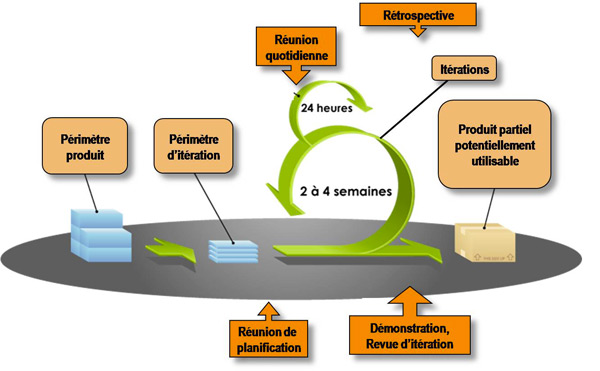
\includegraphics[width=34em]{scrum-agiles.jpg}


\newpage

\begin{itemize}
\item \textbf{Planification du Sprint} (Sprint = itération) : au cours de cette réunion, l’équipe de développement sélectionne les éléments prioritaires du « Product Backlog » (liste ordonnancée des exigences fonctionnelles et non fonctionnelles du projet) qu’elle pense pouvoir réaliser au cours du sprint (en accord avec le « Product Owner »).
\item \textbf{Revue de Sprint} : au cours de cette réunion qui a lieu à la fin du sprint, l’équipe de développement présente les fonctionnalités terminées au cours du sprint et recueille les feedbacks du Product Owner et des utilisateurs finaux. C’est également le moment d’anticiper le périmètre des prochains sprints et d’ajuster au besoin la planification de release (nombre de sprints restants).
\item \textbf{Rétrospective de Sprint} : la rétrospective qui a généralement lieu après la revue de sprint est l’occasion de s’améliorer (productivité, qualité, efficacité, conditions de travail, etc) à la lueur du « vécu » sur le sprint écoulé (principe d’amélioration continue).
\item \textbf{Mêlée quotidienne} : il s’agit d’une réunion de synchronisation de l’équipe de développement qui se fait debout (elle est aussi appelée « stand up meeting ») en 15 minutes maximum au cours de laquelle chacun répond principalement à 3 questions : « Qu’est ce que j’ai terminé depuis la dernière mêlée ? Qu’est ce que j’aurai terminé d’ici la prochaine mêlée ? Quels obstacles me retardent ? »
\end{itemize}



\section{Organisation et responsabilités :}

Lors de la première et la troisième partie du projet, qui consistent au développement de différentes applications, chaque membre de l'équipe sera assigné un rôle particulier :\\

\begin{tabular}{l p{15cm}}
\textbf{Développeur :} & responsables de la production du code. Ils aident aussi à la ré-estimation de la charge de travail en fonction de l'avancement du projet. Ces rôles sont tenus par Julien LEGRAS et Pascal EDOUARD. \\
\textbf{Client :}& notamment le «Product Owner», qui porte vision du produit à réaliser et représente généralement le client afin d'assurer l'intermédiaire avec l'équipe. Ce rôle est tenu par Claire SMETS.\\
\textbf{Testeur :}&  responsable de la création des procédures de tests afin de valider le bon fonctionnement des applications développées. Ce rôle est tenu par Mathieu LATIMIER et William BOISSELEAU.\\
\textbf{Coach :}&  notamment le «Srum Master», reste le garant de l'application de la méthodologie Scrum et de l'équipe en termes de communication et le fonctionnement. Ce rôle est tenu par Pascal EDOUARD.
\end{tabular}

\newpage

\section{Organigramme des tâches :}
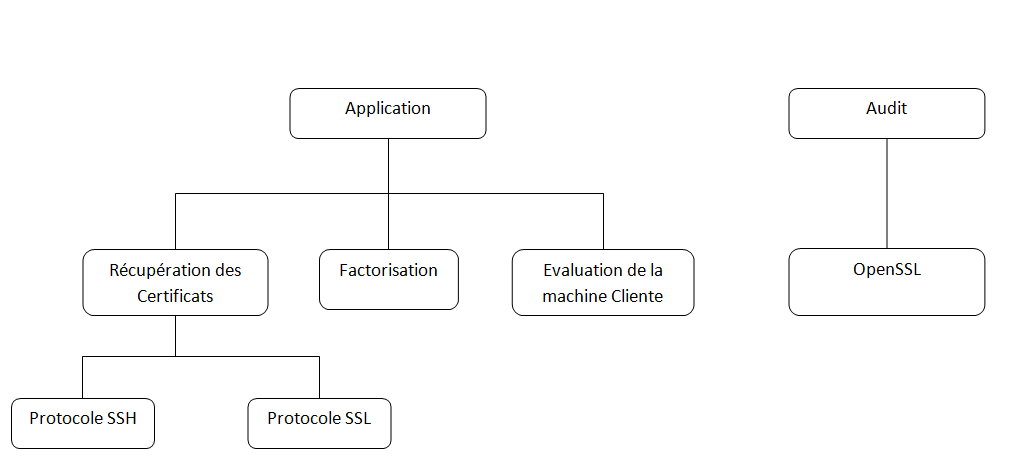
\includegraphics[width=45em]{organigramme.png}

\section{Evaluation du projet :}

L'approche Scrum commence par lister les exigences du client afin de produire le « Product Backlog ». On définit une unité de coût (en terme de complexité) avec la colonne Estimation. Elle permet de faciliter l'ordonnancement du Product Backlog, la planification des sprints et des releases.


\section{Dimensionnement des moyens :}

Nous avons besoin, pour ce projet, d'une bonne connexion internet afin de récupérer le maximum de certificats avec le minimum de perte de connexion possible. Une machine moyenne (normale) en termes de performance est nécessaire pour cette partie. Cependant, l'application de factorisation des moduli nécessite quelque chose de beaucoup plus puissant en termes de disque, mémoire et calcul de processeur. Nos possibilités d'obtenir un serveur de cette taille peuvent varier comme suit :
\begin{enumerate}
\item Serveur local de l'université,
\item Serveur de calcul au CRIHAN,
\item Serveur Amazon à un prix raisonnable.
\end{enumerate}

Le code source ainsi que les différents documents produits sont stockés sur le serveur git : \\ (https://github.com/RandomGuys)

\newpage

\section{Description des tâches :}

\begin{tabular}{|c|c|r|l|}
\hline
&&\textbf{Tâche} & \textbf{Description}\\
\hline
\multirow{13}{*}{\begin{sideways}\textbf{Sprint 1}\end{sideways}}&\multirow{6}{*}{\textbf{App. RC}}
&  1 & Récupération de la liste des adresses IP des serveurs\\
&& 2 & Mise en place des procédures de test			\\
&& 3 & Mise en place d'un client SSH simple			\\
&& 4 & Mise en place d'un client SSL/TLS simple		\\
&& 5 & Récupération des certificats SSL/TLS 		\\
&& 6 & Stockage des certificats SSL/TLS				\\
\cline{2-4}
&\multirow{6}{*}{\textbf{App. F}}
&  7 &  Extraction des clefs des certificats		\\
&& 8 &  Développement des arbres de produits		\\
&& 9 &  Développement des arbres de restes			\\
&& 10 &  Mise en évidence des facteurs communs		\\
&& 11 &  Tests										\\
&& 12 &  Débogage									\\
&& 13 &  Première livraison cliente					\\
&& 14 &  Corrections post-livraison								\\
\cline{1-4}
\multirow{8}{*}{\begin{sideways}\textbf{Sprint 2}\end{sideways}}&\multirow{8}{*}{\textbf{OpenSSL}}
&  15 &  Lister les fonctions d'OpenSSL à auditer\\
&& 16 &  Lister les standards utilisés par chaque fonction à auditer\\
&& 17 &  Mettre en place la page web\\
&& 18 &	 Auditer les fonctions d'OpenSSL listées\\
&& 19 &  Lister les tests et failles existantes\\
&& 20 &  Présenter les clefs communs sur le site\\
&& 21 &  Présenter le résultat de l'audit sur le site\\
&& 22 &  Deuxième livraison cliente\\
&& 23 &  Corrections post-livraison\\
\hline

\multirow{7}{*}{\begin{sideways}\textbf{Sprint 3}\end{sideways}}&\multirow{7}{*}{\textbf{App. Eva}}
&  24 & Lister les critères à vérifier sur une machine cliente\\
&& 25 & Développer la page de connexion client\\
&& 26 & Récupération des données du navigateur\\
&& 27 & Évaluer chaque critère de la machine cliente\\
&& 28 & Présenter les résultats de l'évaluation sur la page web\\
&& 29 & Tests et débeugage\\
&& 30 & Troisième livraison cliente\\\hline

\end{tabular}

\vspace{0.5cm}
\begin{tabular}{|c|c|c|c|c|c|c|c|}
\hline
&\textbf{\No Tâche}&\textbf{Début} & \textbf{Fin} & \textbf{Durée} & \textbf{Effectif} & \textbf{Charge} & \textbf{Ressources}\\
\hline
\multirow{13}{*}{\begin{sideways}\textbf{Sprint 1}\end{sideways}}
&1  		& 20/1/2014 	& 21/1/2014 		& 2		& 1 		& 2			& Julien\\
\cline{2-8}
&2  		& 20/1/2014 	& 23/1/2014 		& 4 	& 2 		& 8			& William, Mathieu\\
\cline{2-8}
&3  		& 20/1/2014 	& 21/1/2014 		& 2 	& 2 		& 4			& Pascal, Claire\\
\cline{2-8}
&4  		& 22/1/2014 	& 23/1/2014 		& 2 	& 1 		& 2			& Julien\\
\cline{2-8}
&5  		& 24/1/2014 	& 24/1/2014 		& 1 	& 3 		& 3			& Julien, Claire, Pascal\\
\cline{2-8}
&6  		& 27/1/2014 	& 27/1/2014 		& 1 	& 3			& 3 		& Julien, Claire, Pascal\\
\cline{2-8}
&7  		& 24/1/2014 	& 24/1/2014 		& 1 	& 2 		& 2			& Mathieu, William\\
\cline{2-8}
&8  		& 24/1/2014 	& 27/1/2014 		& 1.5 	& 2 		& 3			& Mathieu, Pascal\\
\cline{2-8}
&9  		& 24/1/2014 	& 27/1/2014 		& 1 	& 2 		& 3			& Claire, William\\
\cline{2-8}
&10  		& 28/1/2014 	& 30/1/2014 		& 2.5 	& 2 		& 5			& Claire, William\\
\cline{2-8}
&11  		& 30/1/2014 	& 3/2/2014 			& 3 	& 2 		& 5			& William, Pascal, Mathieu\\
\cline{2-8}
&12  		& 30/1/2014 	& 4/2/2014 			& 3 	& 2 		& 8			& Julien, Claire\\
\cline{2-8}
&13  		& 5/2/2014 		& 5/2/2014 			& 1 	& 5 		& --		& Tous\\
\cline{2-8}
&14  		& 6/2/2014 		& 6/2/2014 			& 1 	& 2 		& 2
		& Julien, William\\

\hline
&&&&&&&\\
\hline
\multirow{8}{*}{\begin{sideways}\textbf{Sprint 2}\end{sideways}}
&15 		& 6/2/2014 		& 10/2/2014 		& 3		& 3 		& 9			& William, Julien, Mathieu\\
\cline{2-8}
&16 		& 6/2/2014 		& 7/2/2014 			& 2 	& 2 		& 4			& Pascal, Claire\\
\cline{2-8}
&17 		& 10/2/2014 	& 10/2/2014 		& 1 	& 2 		& 2			& Pascal, Claire\\
\cline{2-8}
&18 		& 11/2/2014 	& 17/2/2014 		& 5 	& 2 		& 10		& Claire, Julien\\
\cline{2-8}
&19 		& 11/2/2014 	& 17/2/2014 		& 5 	& 3 		& 15		& Pascal, William, Mathieu\\
\cline{2-8}
&20 		& 18/2/2014 	& 20/2/2014 		& 3 	& 3 		& 9			& Claire, Pascal, Mathieu\\
\cline{2-8}
&21 		& 18/2/2014 	& 19/2/2014 		& 2 	& 2 		& 4			& Julien, William\\
\cline{2-8}
&22 		& 21/2/2014 	& 21/2/2014 		& 1 	& 5 		& --		& Tous\\
\cline{2-8}
&23 		& 24/2/2014 	& 25/2/2014 		& 2 	& 2 		& 4
		& Pascal, Mathieu\\
\hline
\end{tabular}
\\ \\

Les sprints 1 et 2 sont les parties indispensable. Lors de la répartition des tâches, nous avons donc opté pour la méthode du Planning Poker le mercredi 15 janvier 2014, pour calculer les charges de chaque tâche en équipe et les effectifs nécessaires correspondants. Nous avons donc pu connaître le délais nécessaire pour terminer les 2 premiers sprints.
\\

La date de soutenance du projet étant le vendredi 28 février, la dernière semaine sera plutôt dédié à la rédaction du rapport et préparation de la soutenance. Cependant, dans le cas où nous nous trouvons en avance par rapport aux dates fixées des deux premiers sprint, nous pourrons envisager de considerer le troisième sprint\footnote{Ceci explique pourquoi les charges du troisième sprint furent calculées et ajoutées dans ce tableau}, et dans ce cas seulement.
\\ \\

\newpage

\section{Plan de développement :}

\begin{center}
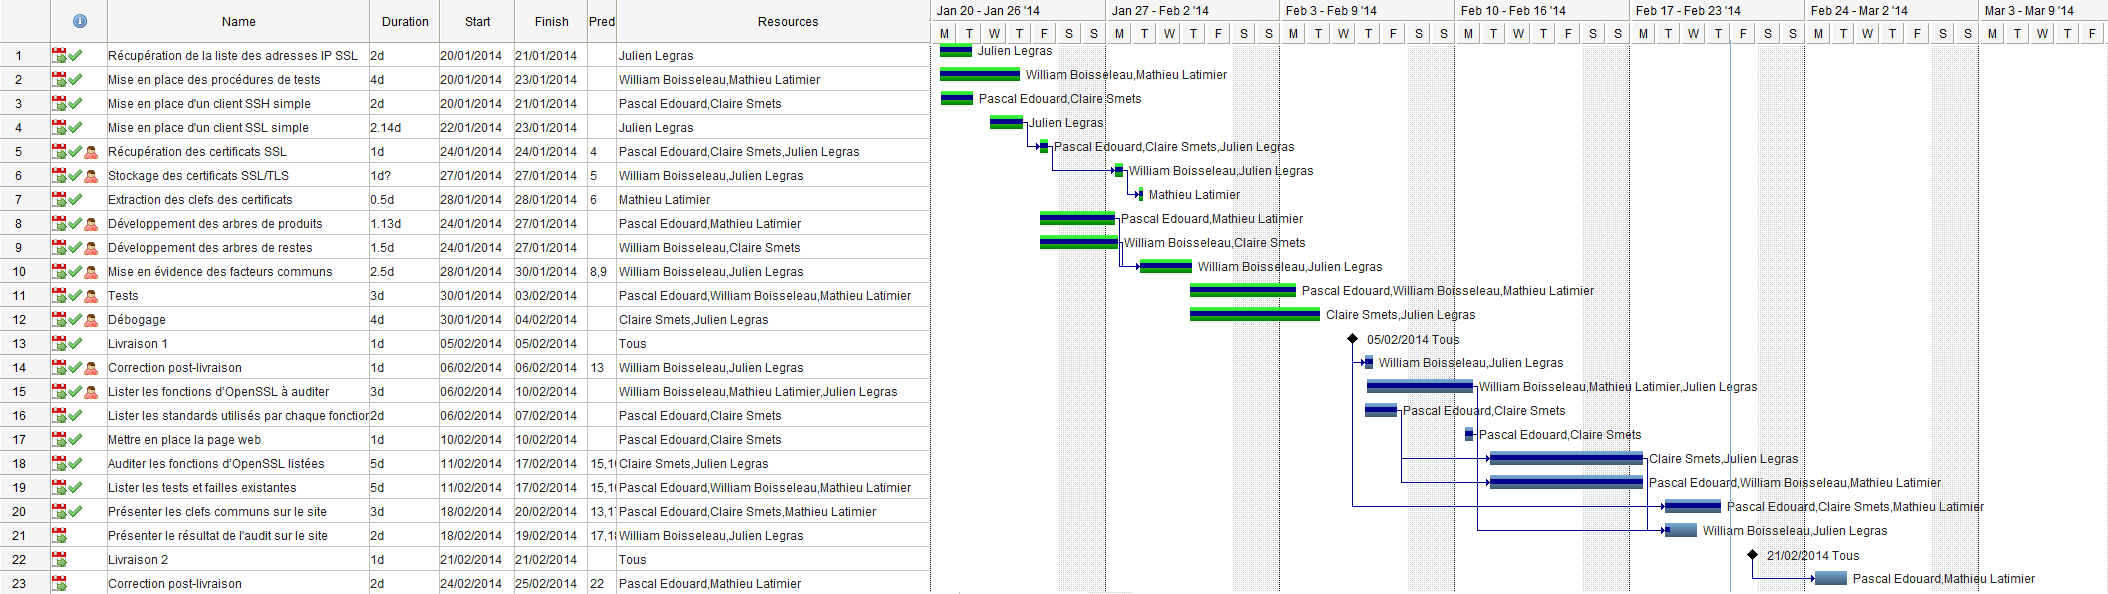
\includegraphics[angle=90,height=22.5cm]{gantt-chart_v1.png}
\end{center}

\newpage



Un outil en ligne, Teambox (récemment renommé en Readbooth) sera utilisé pour gérer la répartition des tâches et suivre leur évolution. Teambox offre une interface permettant de voir ses tâches en cours. La convention utilisée par Teambox, une tâche est assignée à une personne uniquement mais peut avoir plusieurs "watchers" (les personnes qui seront notifiées lors d'un changement ou modification apportées sur la tâche) alors que notre plan de développement précise que plusieurs membres de l'équipe peut travailler sur la même tâche. De ce fait, pour chaque tâche, une personne sera désigné comme responsable de la tache et autres seront donc les "watchers" mais seront toujours capable de modifier la tâche (ajouter des commentaires, modifier son état, ...).

\section{Gestion de la documentation :}
Les documents de référence pour la gestion de ce projet seront disponibles au format pdf sur le serveur git. \\

Chaque membre est responsable d'un document livrable, qui évolue au fil du projet et sera incrémenté par un numéro de version :\\ \\
\begin{tabular}{ll}
–	La Spécification Technique du Besoin 	& : Claire SMETS\\
–	Le Document d'Architecture Logicielle 	& : Julien LEGRAS\\
–	L'Analyse des Risques 					& : Pascal EDOUARD\\
–	Le Cahier des Recettes 					& : Mathieu LATIMIER et William BOISSELEAU\\
–	Le Plan de Développement 				& : Pascal EDOUARD\\
\end{tabular}
\\ \\

L'ensemble du groupe devra se tenir au courant de l'évolution de chaque document. De plus, après chaque réunion avec le client, un compte-rendu sera rédigé et validé par l'équipe avant d'être soumis au client, qui pourra ensuite le valider. Le compte-rendu sera accessible sur le dépôt de documents git.
\\
Ce dépôt permettra à l'équipe de suivre l'évolution des documents (livrables, compte-rendu, ...) ainsi que les fichiers de scripts développés durant le projet. En cas de perte des données, il sera possible de retrouver une ancience version et limiter les pertes.
\\ \\
Une intégration Git - Teambox est également possible afin de suivre la gestion de la documentation et le plan de développement plus facilement. En effet, la fonction de hooks de Git permet de rajouter un commentaire à chaque fois qu'un commit (sauvegarde d'une modification directement sur le dépot) est effectué par l'un des membres de l'équipe.
\end{document}
